\chapter{Risultati Sperimentali}
\label{ch:risultati}

I benchmark sono stati condotti su due mappe (\textbf{Mappa~A} e \textbf{Mappa~B}),
ciascuna con due batterie di test:

\begin{enumerate}
  \item \textbf{Test esaustivo (32.768 simulazioni)} --- tutte le combinazioni di 4 strategie
        (Frontier, Greedy, Sector, Repulsion), raggi di visione $v_r \in \{2,3\}$ e raggio di
        comunicazione fisso $c_r = 2$, per un team di 5 agenti. Limite: 500 tick.
  \item \textbf{Test randomizzato (100$\times$3 seed)} --- 100 preset casuali con 5 strategie
        (incluso Smart Random Walk), $v_r \in \{1,2,3\}$, $c_r \in \{1,2\}$, ripetuti su tre seed
        indipendenti (42, 43, 44) per valutare la robustezza statistica. Limite: 500 tick.
\end{enumerate}

\paragraph{Nota sulla configurazione del test esaustivo.}
Smart Random Walk non \`e stato incluso nel test esaustivo (32.768 simulazioni) poich\'e
la sua aggiunta come quinta strategia avrebbe moltiplicato il numero di combinazioni in modo
esponenziale, rendendo il benchmark computazionalmente infatibile. Abbinato ai 2 raggi di
visione e al raggio di comunicazione fisso, il costo temporale totale sarebbe stato inaccettabile.
Per questo motivo, \`e stata scelta Random Walk come sacrificio dalla configurazione esaustiva.
Nonostante la sua componente stocastica, Random Walk dimostrava efficienza comparabile alle altre
strategie; tuttavia, era meno versatile nei contesti eterogenei, rendendone la scelta pi\`u
accettabile. Smart Random Walk rimane incluso nel test randomizzato dove la ricchezza dei dati
permette comunque di valutarne il comportamento.

%% ═════════════════════════════════════════════════════════════════════════════
\section{Mappa A}
%% ═════════════════════════════════════════════════════════════════════════════

\subsection{Test esaustivo --- 32.768 simulazioni}

Sono state eseguite 32.768 simulazioni in circa 3\,h\,15\,min di tempo CPU.

\begin{itemize}
  \item \textbf{Tasso di completamento}: 96,4\,\% dei preset ha consegnato tutti e 10 gli oggetti
        (31.602 su 32.768). Il tasso medio di consegna \`e $\overline{r} = 0{,}990$.
  \item \textbf{Tick medi di completamento}: $\overline{T} = 162{,}9$ tick
        (calcolati solo sui preset completati al 100\,\%). Il miglior preset ha
        completato in soli 77 tick.
  \item \textbf{Energia media}: $\overline{E} = 173{,}1$ unit\`a consumate per agente.
\end{itemize}

\begin{figure}[H]
  \centering
  \includegraphics[width=0.75\textwidth]{../../benchmarks/A/32k_sim/Configurazione.png}
  \caption{Configurazione della Mappa~A utilizzata nel test esaustivo.}
  \label{fig:confA-32k}
\end{figure}

\begin{figure}[H]
  \centering
  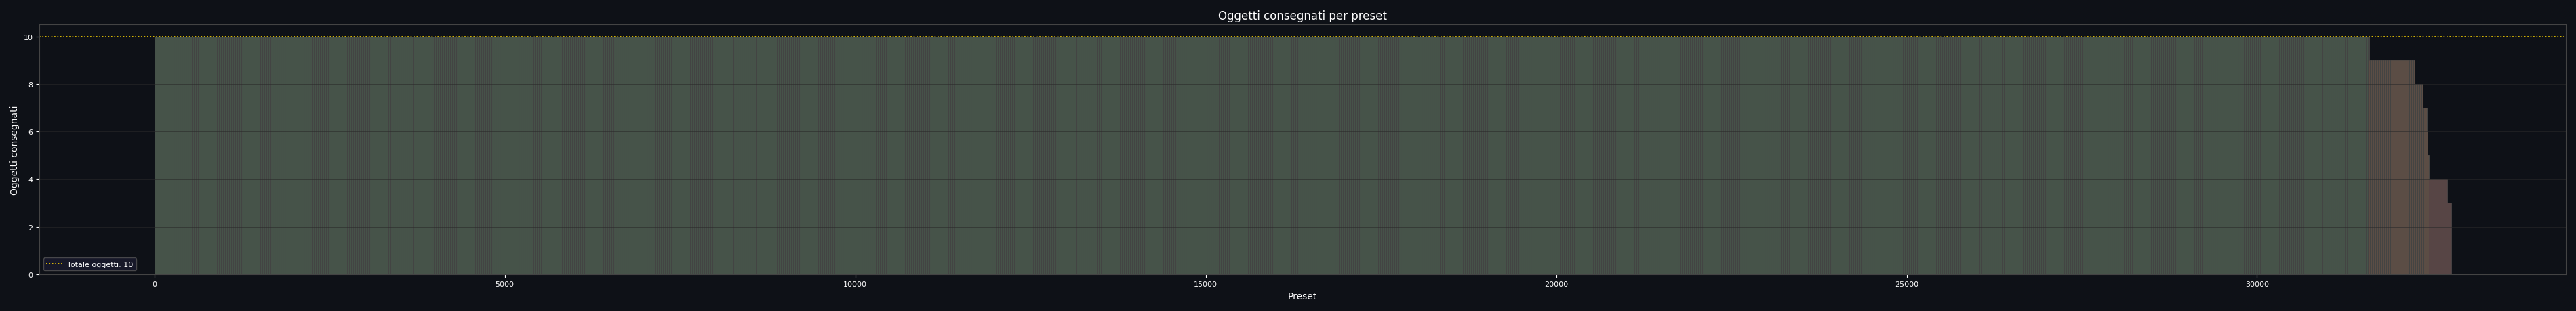
\includegraphics[width=\textwidth]{../../benchmarks/A/32k_sim/Images/plot/grafico_oggetti_consegnati.png}
  \caption{Mappa~A --- 32k sim: distribuzione degli oggetti consegnati per preset. Tasso di completamento: 96,4\%}
  \label{fig:A32k-oggetti}
\end{figure}

\begin{figure}[H]
  \centering
  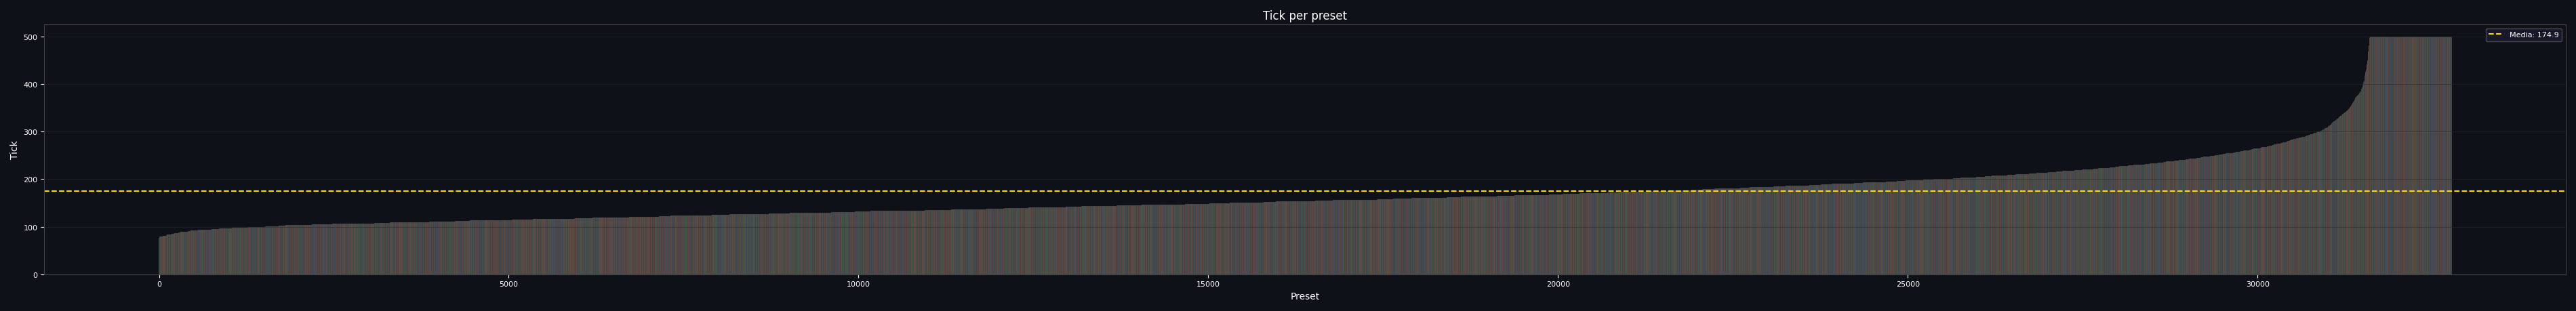
\includegraphics[width=\textwidth]{../../benchmarks/A/32k_sim/Images/plot/grafico_tick_completamento.png}
  \caption{Mappa~A --- 32k sim: tick di completamento per preset. Tick medi: 174,9. Energia media consumata: 173,1 unit\`a.}
  \label{fig:A32k-tick}
\end{figure}

\begin{figure}[H]
  \centering
  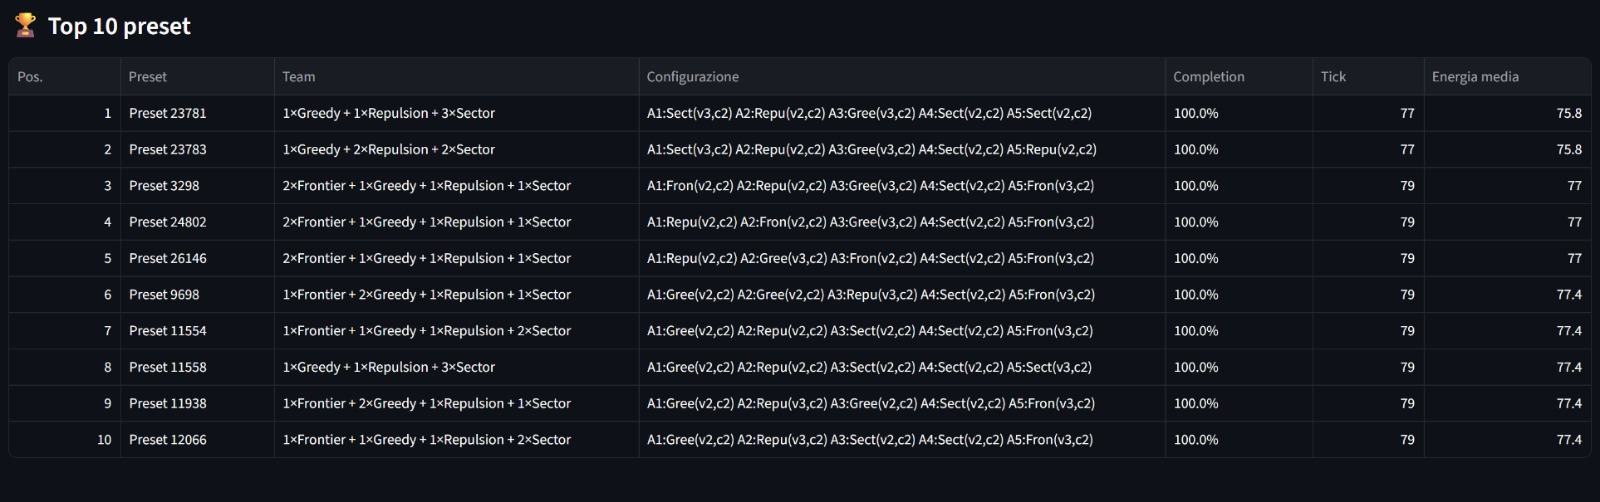
\includegraphics[width=0.92\textwidth]{../../benchmarks/A/32k_sim/Images/tabelle/tabellaTop10.jpeg}
  \caption{Mappa~A --- 32k sim: classifica dei 10 migliori preset per tick di completamento.}
  \label{fig:A32k-top10}
\end{figure}

\begin{table}[H]
\centering
\caption{Mappa~A --- Top~10 preset nel test esaustivo (32k simulazioni).}
\label{tab:A32k-top10}
\small
\begin{tabular}{c l l c c}
\toprule
\textbf{\#} & \textbf{Preset} & \textbf{Composizione team} & \textbf{Tick} & $\overline{E}$ \\
\midrule
1  & 23781 & Sect($v_3$) Repu($v_2$) Gree($v_3$) Sect($v_2$) Sect($v_2$) & 77  & 75{,}8  \\
2  & 23783 & Sect($v_3$) Repu($v_2$) Gree($v_3$) Sect($v_2$) Repu($v_2$) & 77  & 75{,}8  \\
3  & 3298  & Fron($v_2$) Repu($v_2$) Gree($v_3$) Sect($v_2$) Fron($v_3$) & 79  & 77{,}0  \\
4  & 24802 & Repu($v_2$) Fron($v_2$) Gree($v_3$) Sect($v_2$) Fron($v_3$) & 79  & 77{,}0  \\
5  & 26146 & Repu($v_2$) Gree($v_3$) Fron($v_2$) Sect($v_2$) Fron($v_3$) & 79  & 77{,}0  \\
6  & 9698  & Gree($v_2$) Gree($v_2$) Repu($v_3$) Sect($v_2$) Fron($v_3$) & 79  & 77{,}4  \\
7  & 11554 & Gree($v_2$) Repu($v_2$) Sect($v_2$) Sect($v_2$) Fron($v_3$) & 79  & 77{,}4  \\
8  & 11558 & Gree($v_2$) Repu($v_2$) Sect($v_2$) Sect($v_2$) Sect($v_3$) & 79  & 77{,}4  \\
9  & 11938 & Gree($v_2$) Repu($v_3$) Gree($v_2$) Sect($v_2$) Fron($v_3$) & 79  & 77{,}4  \\
10 & 12066 & Gree($v_2$) Repu($v_3$) Sect($v_2$) Sect($v_2$) Fron($v_3$) & 79  & 77{,}4  \\
\bottomrule
\end{tabular}

\vspace{4pt}
{\footnotesize Legenda: Fron = Frontier, Gree = Greedy, Sect = Sector,
Repu = Repulsion. $v_k$ = raggio di visibilit\`a $k$. $c_r = 2$ per tutti.}
\end{table}

%% ── 100×3 ────────────────────────────────────────────────────────────────────
\subsection{Test randomizzato --- 100$\times$3 seed}

La media complessiva sui tre seed \`e:

\begin{itemize}
  \item \textbf{Tasso di completamento medio}: 99,6\,\% (96/100 completati per seed~42 e 44, 97/100 per seed~43).
  \item \textbf{Tick medi di completamento}: $\overline{T} = 158{,}5$ tick
        (media dei preset completati al 100\,\% sui tre seed).
  \item \textbf{Energia media}: $\overline{E} = 169{,}0$.
\end{itemize}

\begin{figure}[H]
  \centering
  \includegraphics[width=0.75\textwidth]{../../benchmarks/A/100_sim/Configurazione.png}
  \caption{Configurazione della Mappa~A utilizzata nel test randomizzato.}
  \label{fig:confA-100}
\end{figure}

\subsubsection*{Seed 42}

\begin{figure}[H]
  \centering
  \includegraphics[width=\textwidth]{../../benchmarks/A/100_sim/seed42/Images/plot/grafico_oggetti_consegnati.png}
  \caption{Mappa~A --- seed 42: oggetti consegnati per preset.}
  \label{fig:As42-oggetti}
\end{figure}

\begin{figure}[H]
  \centering
  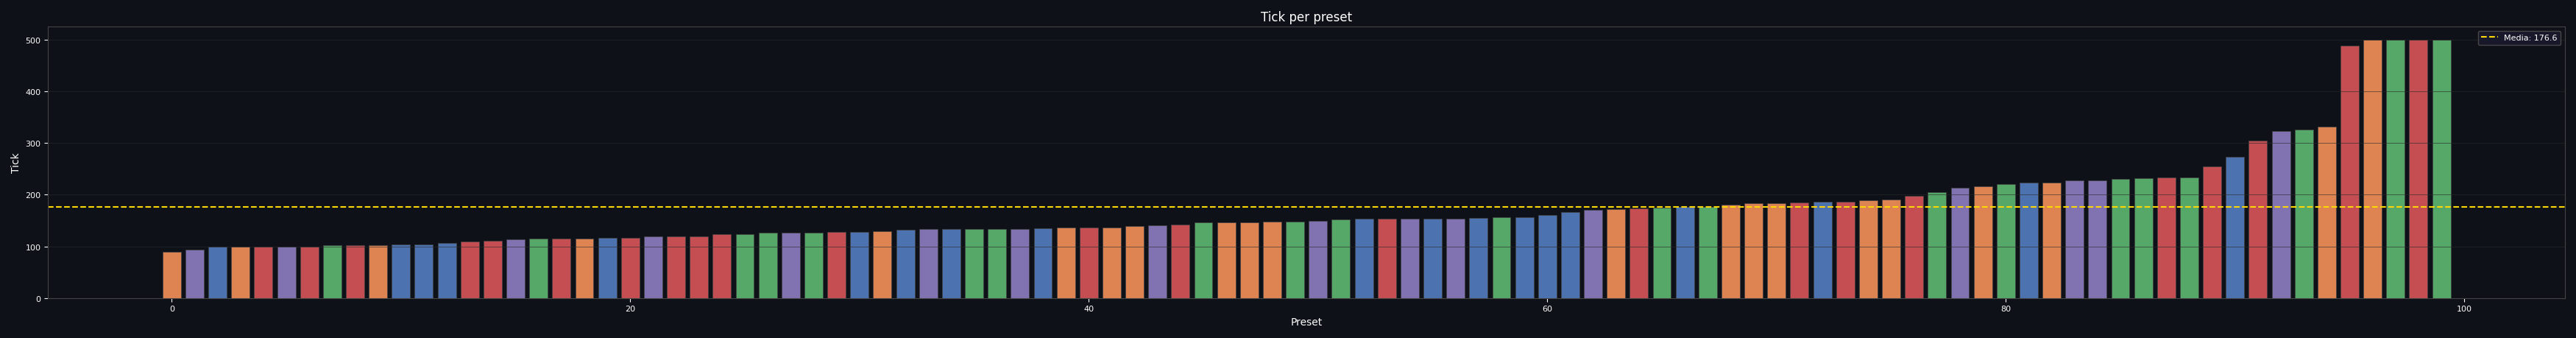
\includegraphics[width=\textwidth]{../../benchmarks/A/100_sim/seed42/Images/plot/grafico_tick_completamento.png}
  \caption{Mappa~A --- seed 42: tick di completamento per preset.}
  \label{fig:As42-tick}
\end{figure}

\begin{figure}[H]
  \centering
  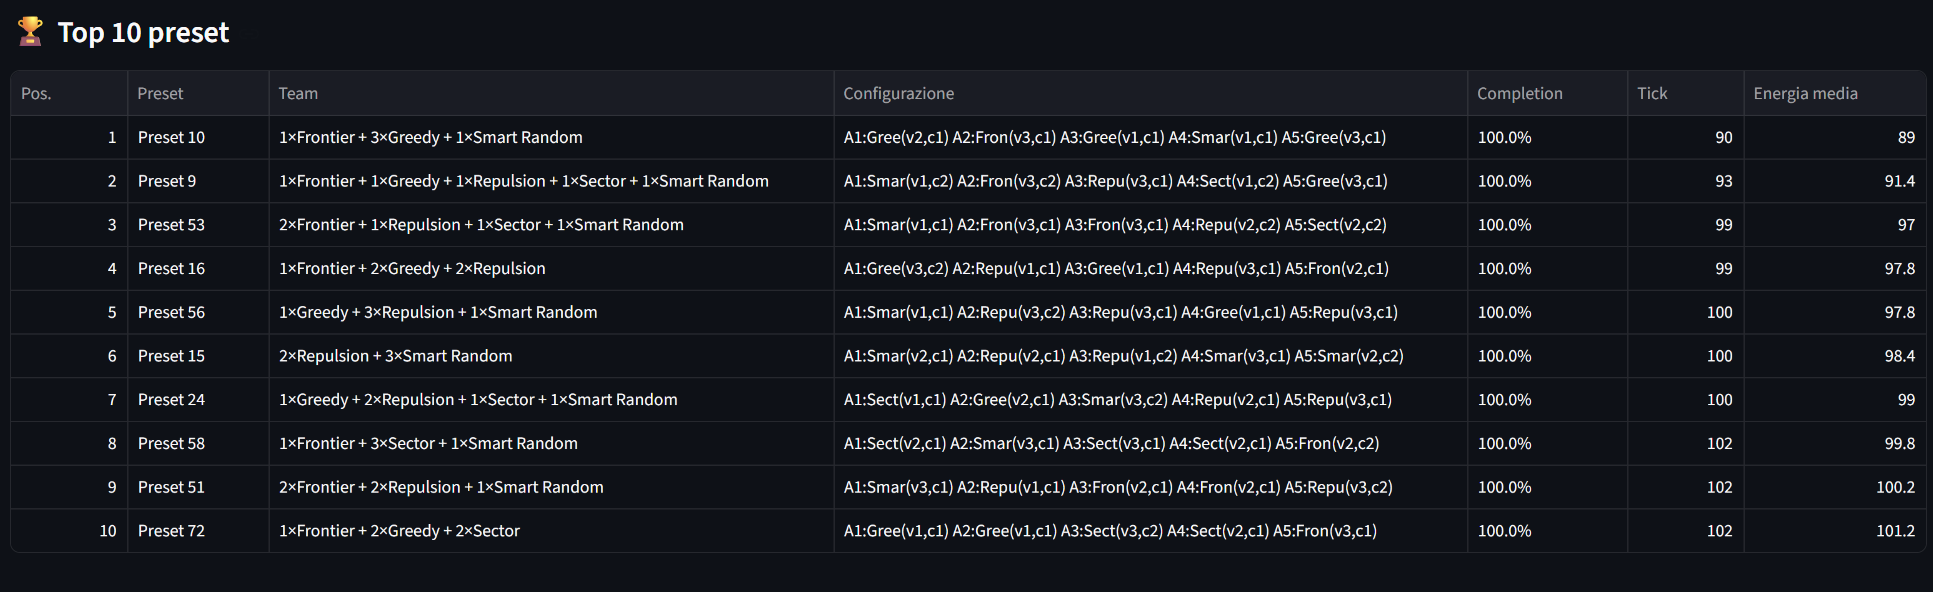
\includegraphics[width=0.92\textwidth]{../../benchmarks/A/100_sim/seed42/Images/tabelle/tabellaTop10.png}
  \caption{Mappa~A --- seed 42: classifica Top~10.}
  \label{fig:As42-top10}
\end{figure}

\subsubsection*{Seed 43}

\begin{figure}[H]
  \centering
  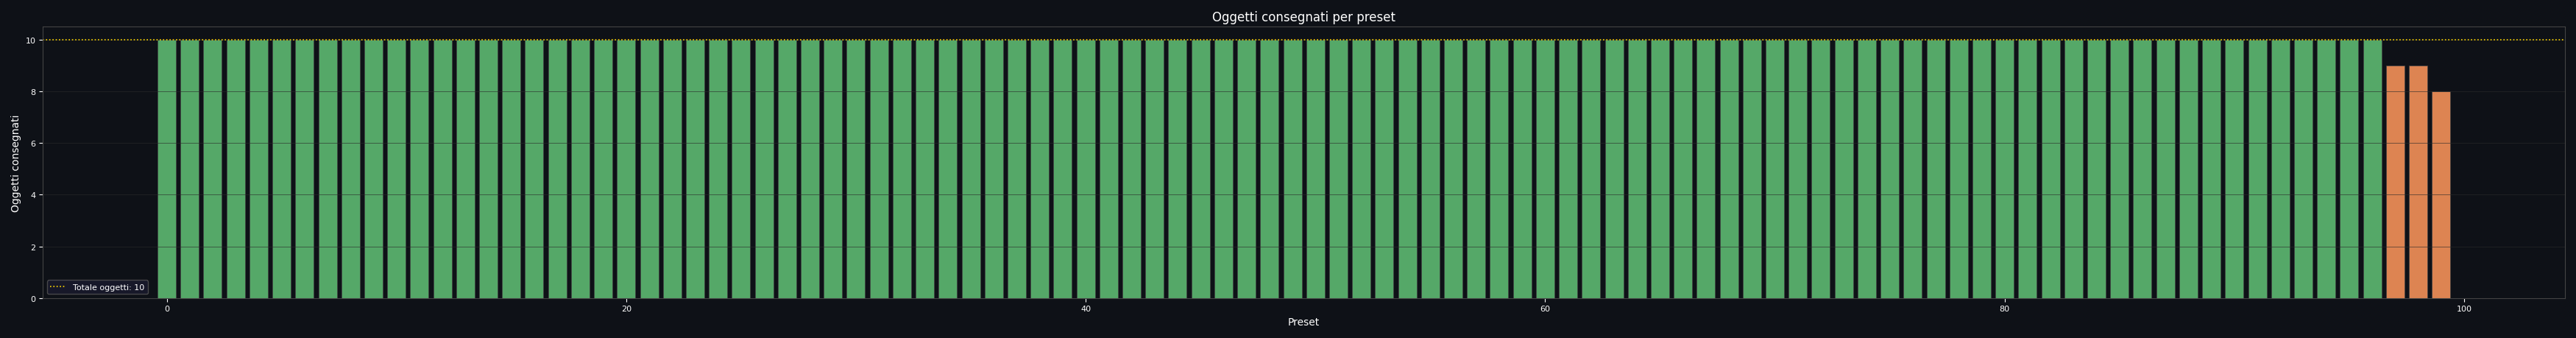
\includegraphics[width=\textwidth]{../../benchmarks/A/100_sim/seed43/Images/plot/grafico_oggetti_consegnati.png}
  \caption{Mappa~A --- seed 43: oggetti consegnati per preset.}
  \label{fig:As43-oggetti}
\end{figure}

\begin{figure}[H]
  \centering
  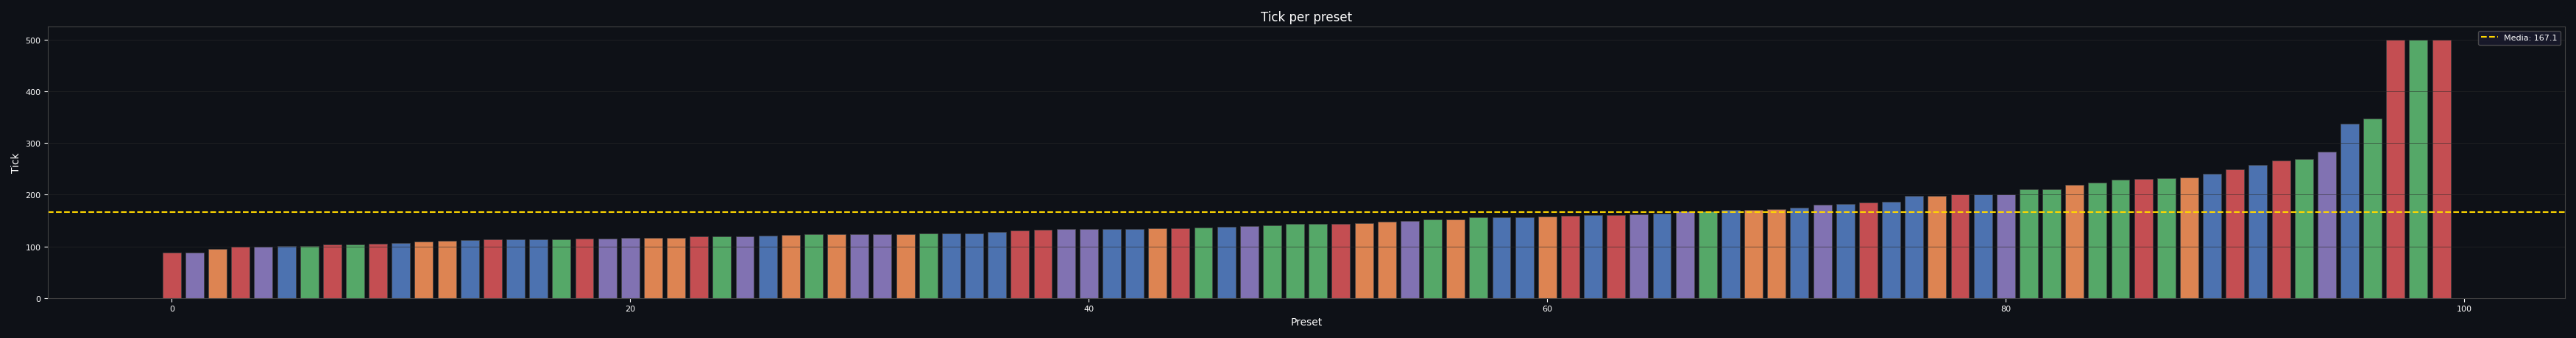
\includegraphics[width=\textwidth]{../../benchmarks/A/100_sim/seed43/Images/plot/grafico_tick_completamento.png}
  \caption{Mappa~A --- seed 43: tick di completamento per preset.}
  \label{fig:As43-tick}
\end{figure}

\begin{figure}[H]
  \centering
  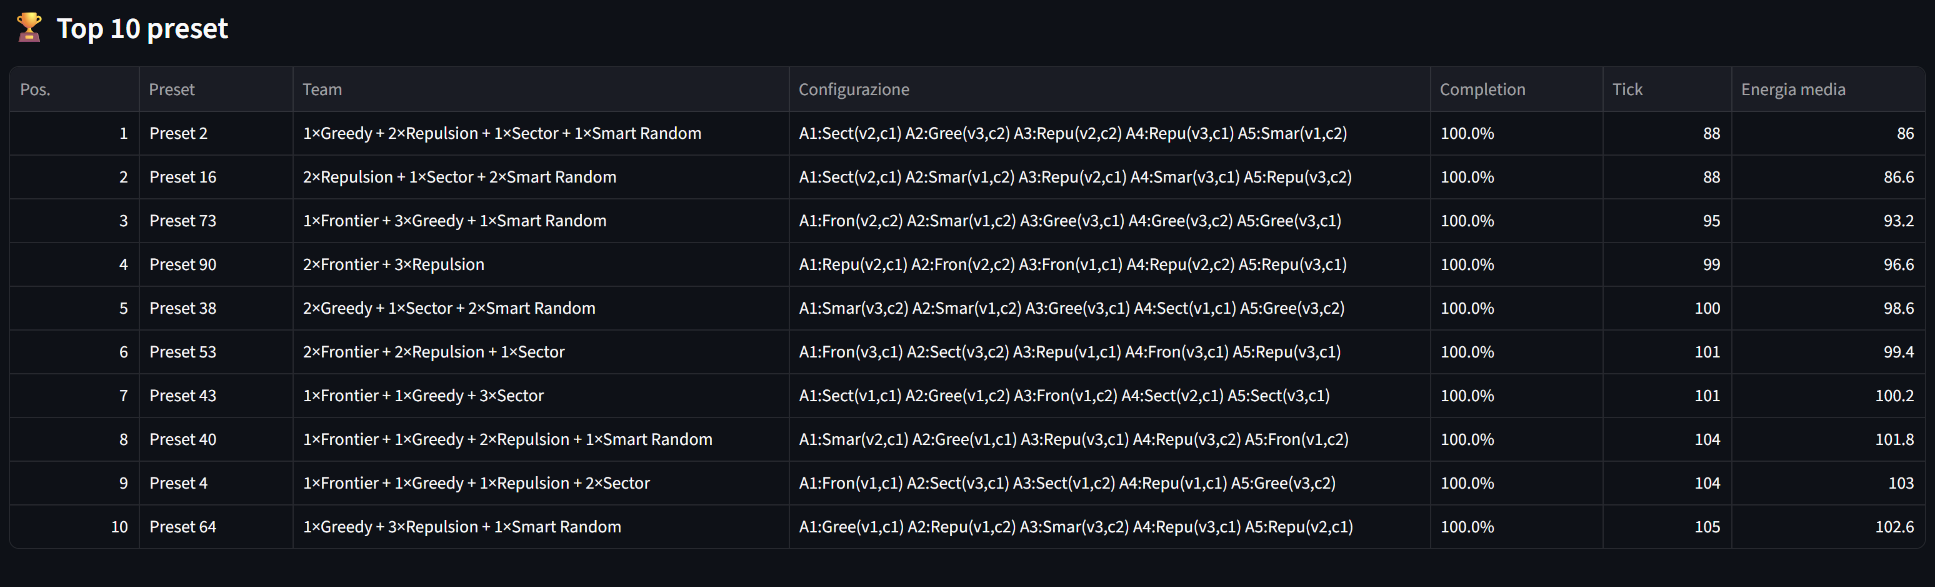
\includegraphics[width=0.92\textwidth]{../../benchmarks/A/100_sim/seed43/Images/tabelle/tabellaTop10.png}
  \caption{Mappa~A --- seed 43: classifica Top~10.}
  \label{fig:As43-top10}
\end{figure}

\subsubsection*{Seed 44}

\begin{figure}[H]
  \centering
  \includegraphics[width=\textwidth]{../../benchmarks/A/100_sim/seed44/Images/plot/grafico_oggetti_consegnati.png}
  \caption{Mappa~A --- seed 44: oggetti consegnati per preset.}
  \label{fig:As44-oggetti}
\end{figure}

\begin{figure}[H]
  \centering
  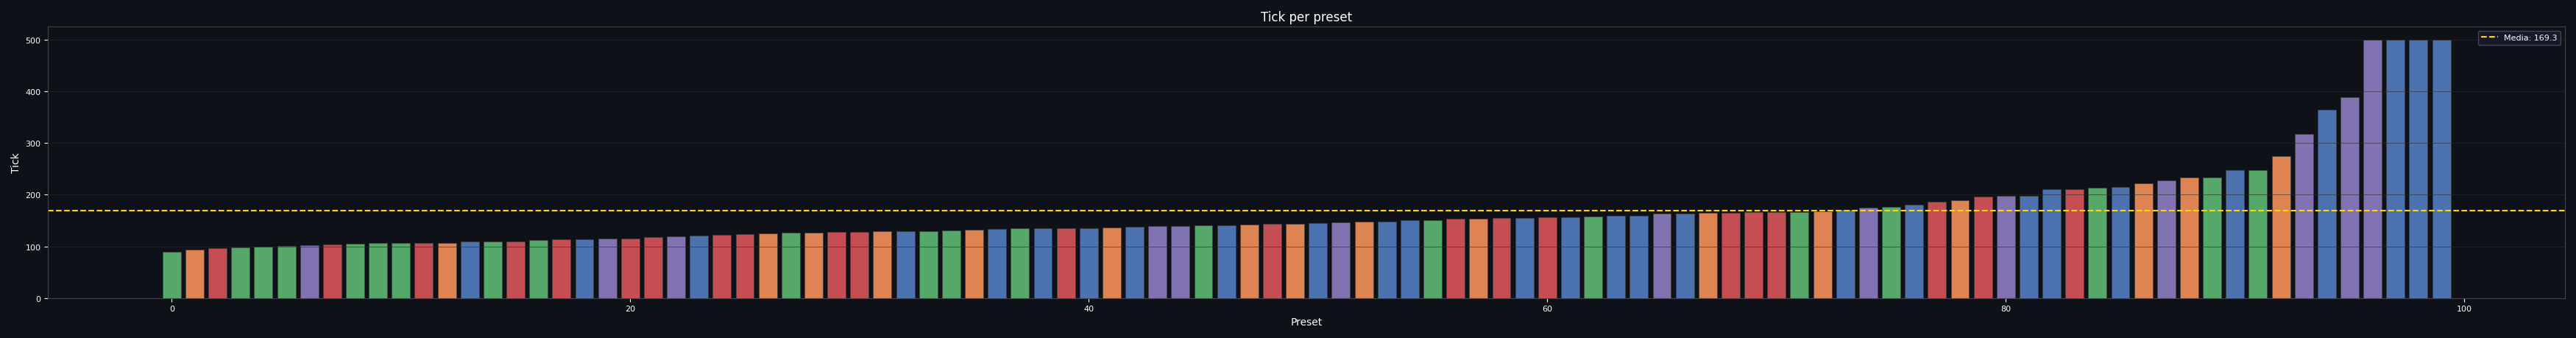
\includegraphics[width=\textwidth]{../../benchmarks/A/100_sim/seed44/Images/plot/grafico_tick_completamento.png}
  \caption{Mappa~A --- seed 44: tick di completamento per preset.}
  \label{fig:As44-tick}
\end{figure}

\begin{figure}[H]
  \centering
  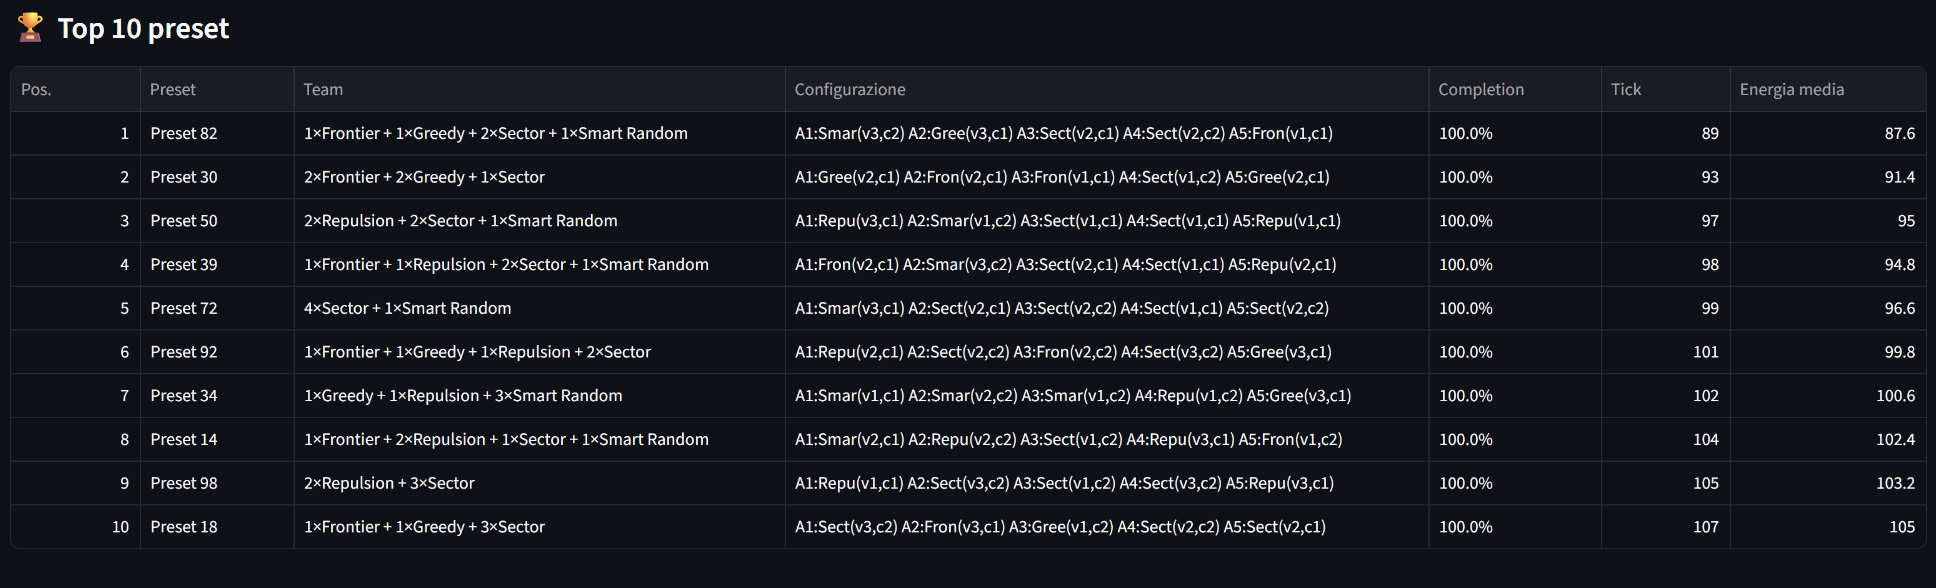
\includegraphics[width=0.92\textwidth]{../../benchmarks/A/100_sim/seed44/Images/tabelle/tabellaTop10.png}
  \caption{Mappa~A --- seed 44: classifica Top~10.}
  \label{fig:As44-top10}
\end{figure}

%% ═════════════════════════════════════════════════════════════════════════════
\section{Mappa B}
%% ═════════════════════════════════════════════════════════════════════════════

\subsection{Test esaustivo --- 32.768 simulazioni}

Tempo CPU totale: circa 2\,h\,30\,min.

\begin{itemize}
  \item \textbf{Tasso di completamento}: 99,6\,\% (32.652 su 32.768).
        $\overline{r} = 0{,}9995$.
  \item \textbf{Tick medi di completamento}: $\overline{T} = 105{,}7$ tick.
        Il miglior preset ha completato in 57 tick.
  \item \textbf{Energia media}: $\overline{E} = 104{,}7$.
\end{itemize}

Rispetto alla Mappa~A, la Mappa~B risulta sensibilmente pi\`u
facile: tasso di completamento pi\`u alto (+3,2~pp), tick medi pi\`u
bassi ($-35\,\%$) e minor consumo energetico ($-40\,\%$).

\begin{figure}[H]
  \centering
  \includegraphics[width=0.75\textwidth]{../../benchmarks/B/32k_sim/Configurazione.png}
  \caption{Configurazione della Mappa~B utilizzata nel test esaustivo.}
  \label{fig:confB-32k}
\end{figure}

\begin{figure}[H]
  \centering
  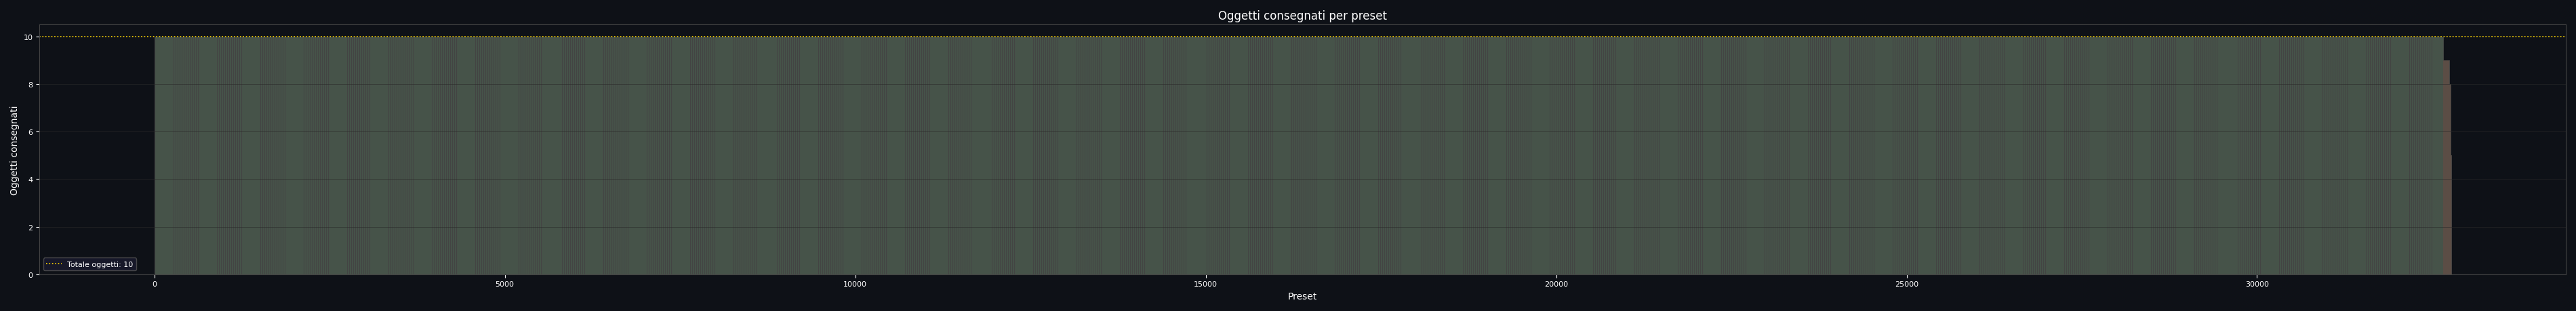
\includegraphics[width=\textwidth]{../../benchmarks/B/32k_sim/Images/plot/grafico_oggetti_consegnati.png}
  \caption{Mappa~B --- 32k sim: distribuzione degli oggetti consegnati per preset. Tasso di completamento: 99,6\%}
  \label{fig:B32k-oggetti}
\end{figure}

\begin{figure}[H]
  \centering
  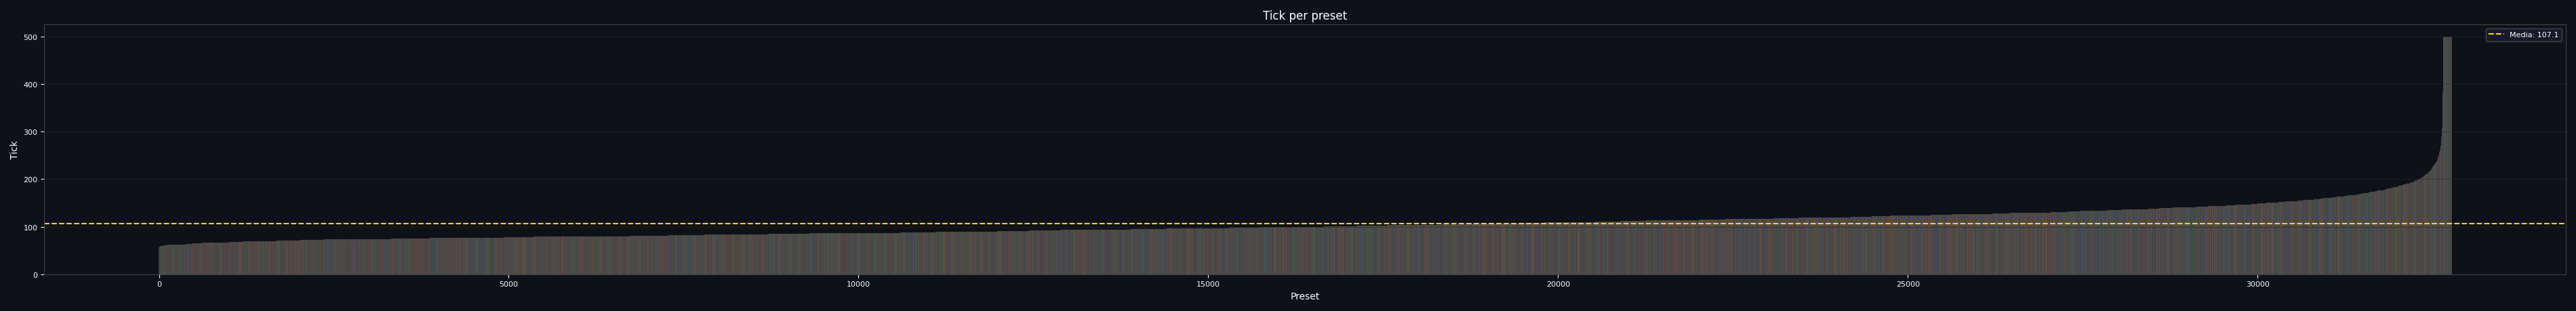
\includegraphics[width=\textwidth]{../../benchmarks/B/32k_sim/Images/plot/grafico_tick_completamento.png}
  \caption{Mappa~B --- 32k sim: tick di completamento per preset. Tick medi: 107,1. Energia media consumata: 104,7 unit\`a.}
  \label{fig:B32k-tick}
\end{figure}

\begin{figure}[H]
  \centering
  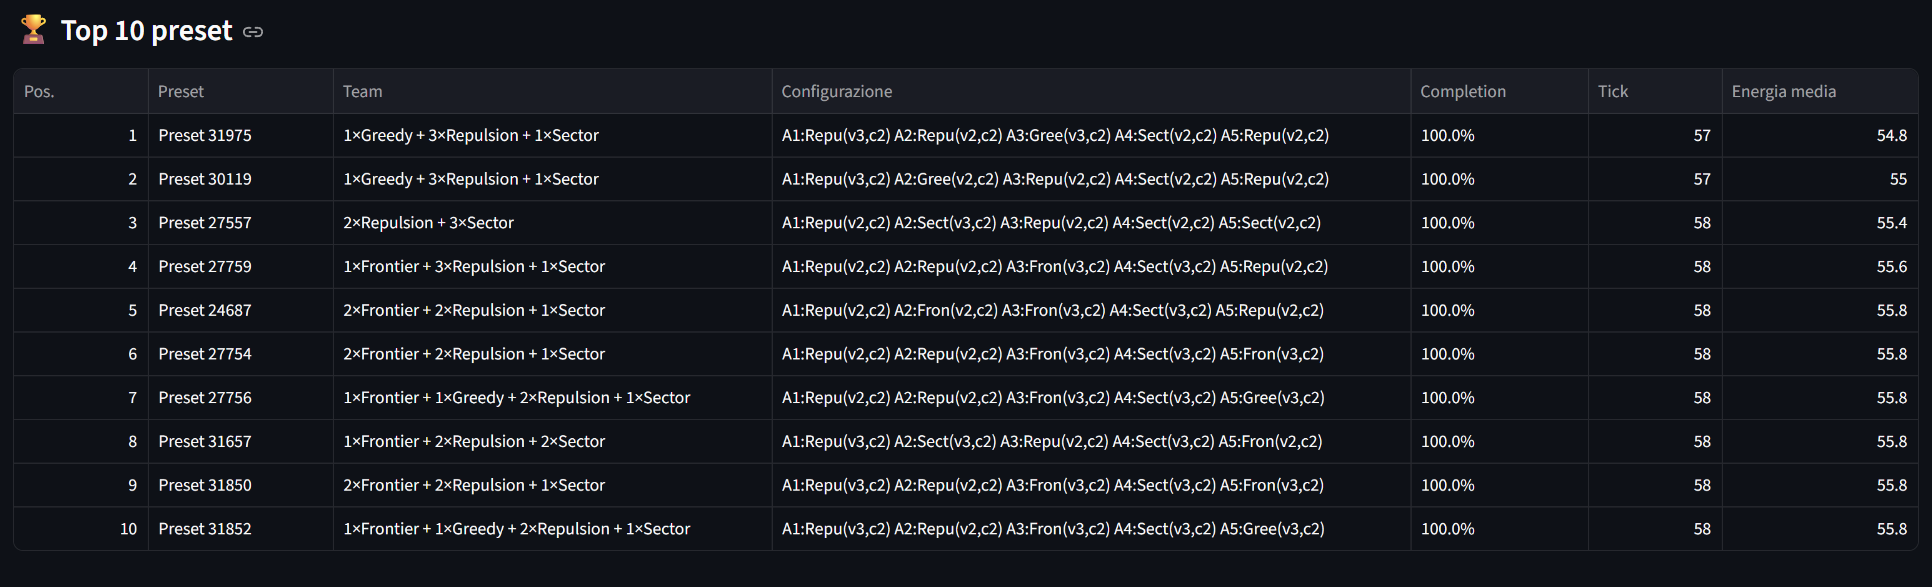
\includegraphics[width=0.92\textwidth]{../../benchmarks/B/32k_sim/Images/tabelle/tabellaTop10.png}
  \caption{Mappa~B --- 32k sim: classifica dei 10 migliori preset per tick di completamento.}
  \label{fig:B32k-top10}
\end{figure}

\begin{table}[H]
\centering
\caption{Mappa~B --- Top~10 preset nel test esaustivo (32k simulazioni).}
\label{tab:B32k-top10}
\small
\begin{tabular}{c l l c c}
\toprule
\textbf{\#} & \textbf{Preset} & \textbf{Composizione team} & \textbf{Tick} & $\overline{E}$ \\
\midrule
1  & 31975 & Repu($v_3$) Repu($v_2$) Gree($v_3$) Sect($v_2$) Repu($v_2$) & 57  & 54{,}8  \\
2  & 30119 & Repu($v_3$) Gree($v_2$) Repu($v_2$) Sect($v_2$) Repu($v_2$) & 57  & 55{,}0  \\
3  & 27557 & Repu($v_2$) Sect($v_3$) Repu($v_2$) Sect($v_2$) Sect($v_2$) & 58  & 55{,}4  \\
4  & 27759 & Repu($v_2$) Repu($v_2$) Fron($v_3$) Sect($v_3$) Repu($v_2$) & 58  & 55{,}6  \\
5  & 24687 & Repu($v_2$) Fron($v_2$) Fron($v_3$) Sect($v_3$) Repu($v_2$) & 58  & 55{,}8  \\
6  & 27754 & Repu($v_2$) Repu($v_2$) Fron($v_3$) Sect($v_3$) Fron($v_3$) & 58  & 55{,}8  \\
7  & 27756 & Repu($v_2$) Repu($v_2$) Fron($v_3$) Sect($v_3$) Gree($v_3$) & 58  & 55{,}8  \\
8  & 31657 & Repu($v_3$) Sect($v_3$) Repu($v_2$) Sect($v_3$) Fron($v_2$) & 58  & 55{,}8  \\
9  & 31850 & Repu($v_3$) Repu($v_2$) Fron($v_3$) Sect($v_3$) Fron($v_3$) & 58  & 55{,}8  \\
10 & 31852 & Repu($v_3$) Repu($v_2$) Fron($v_3$) Sect($v_3$) Gree($v_3$) & 58  & 55{,}8  \\
\bottomrule
\end{tabular}

\vspace{4pt}
{\footnotesize Legenda: Fron = Frontier, Gree = Greedy, Sect = Sector,
Repu = Repulsion. $v_k$ = raggio di visibilit\`a $k$. $c_r = 2$ per tutti.}
\end{table}

%% ── 100×3 ────────────────────────────────────────────────────────────────────
\subsection{Test randomizzato --- 100$\times$3 seed}

La media complessiva sui tre seed \`e:

\begin{itemize}
  \item \textbf{Tasso di completamento medio}: 99,97\,\% (tutti i 100 preset completati
        con seed~42 e 43; 99/100 con seed~44).
  \item \textbf{Tick medi di completamento}: $\overline{T} = 112{,}6$ tick.
  \item \textbf{Energia media}: $\overline{E} = 111{,}6$.
\end{itemize}

\begin{figure}[H]
  \centering
  \includegraphics[width=0.75\textwidth]{../../benchmarks/B/100_sim/Configurazione.png}
  \caption{Configurazione della Mappa~B utilizzata nel test randomizzato.}
  \label{fig:confB-100}
\end{figure}

\subsubsection*{Seed 42}

\begin{figure}[H]
  \centering
  \includegraphics[width=\textwidth]{../../benchmarks/B/100_sim/seed42/Images/plot/grafico_oggetti_consegnati.png}
  \caption{Mappa~B --- seed 42: oggetti consegnati per preset.}
  \label{fig:Bs42-oggetti}
\end{figure}

\begin{figure}[H]
  \centering
  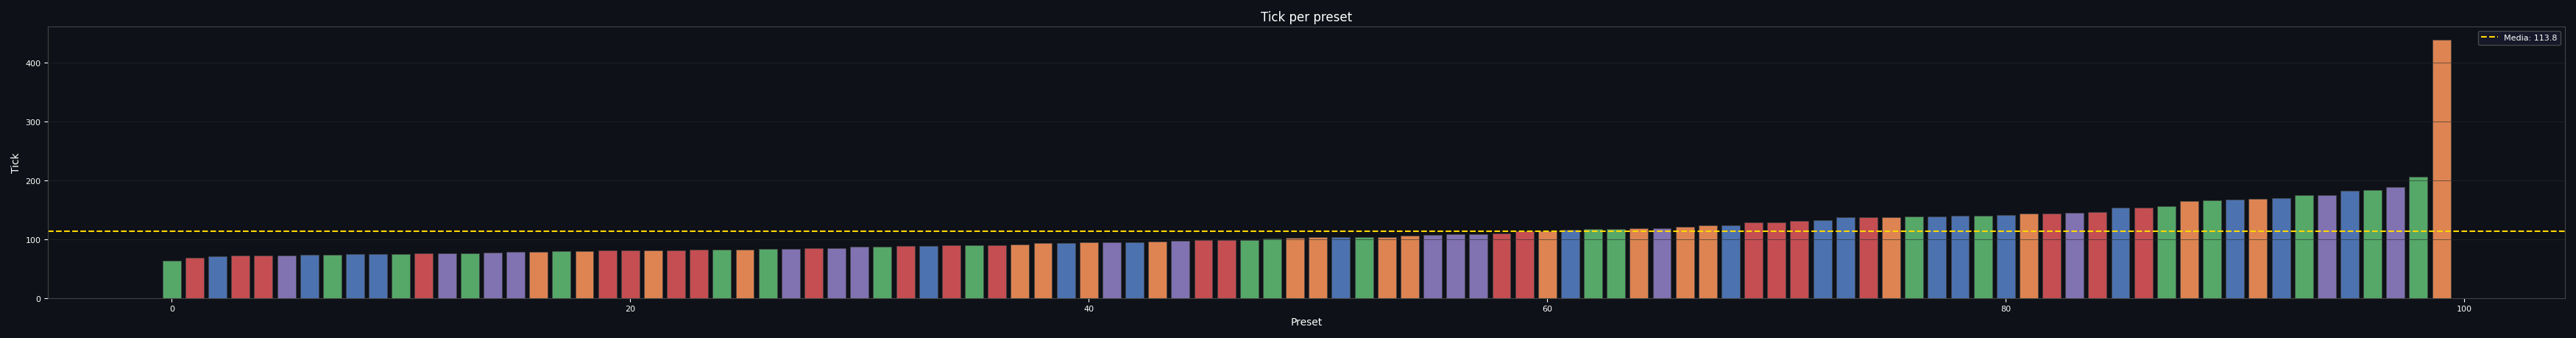
\includegraphics[width=\textwidth]{../../benchmarks/B/100_sim/seed42/Images/plot/grafico_tick_completamento.png}
  \caption{Mappa~B --- seed 42: tick di completamento per preset.}
  \label{fig:Bs42-tick}
\end{figure}

\begin{figure}[H]
  \centering
  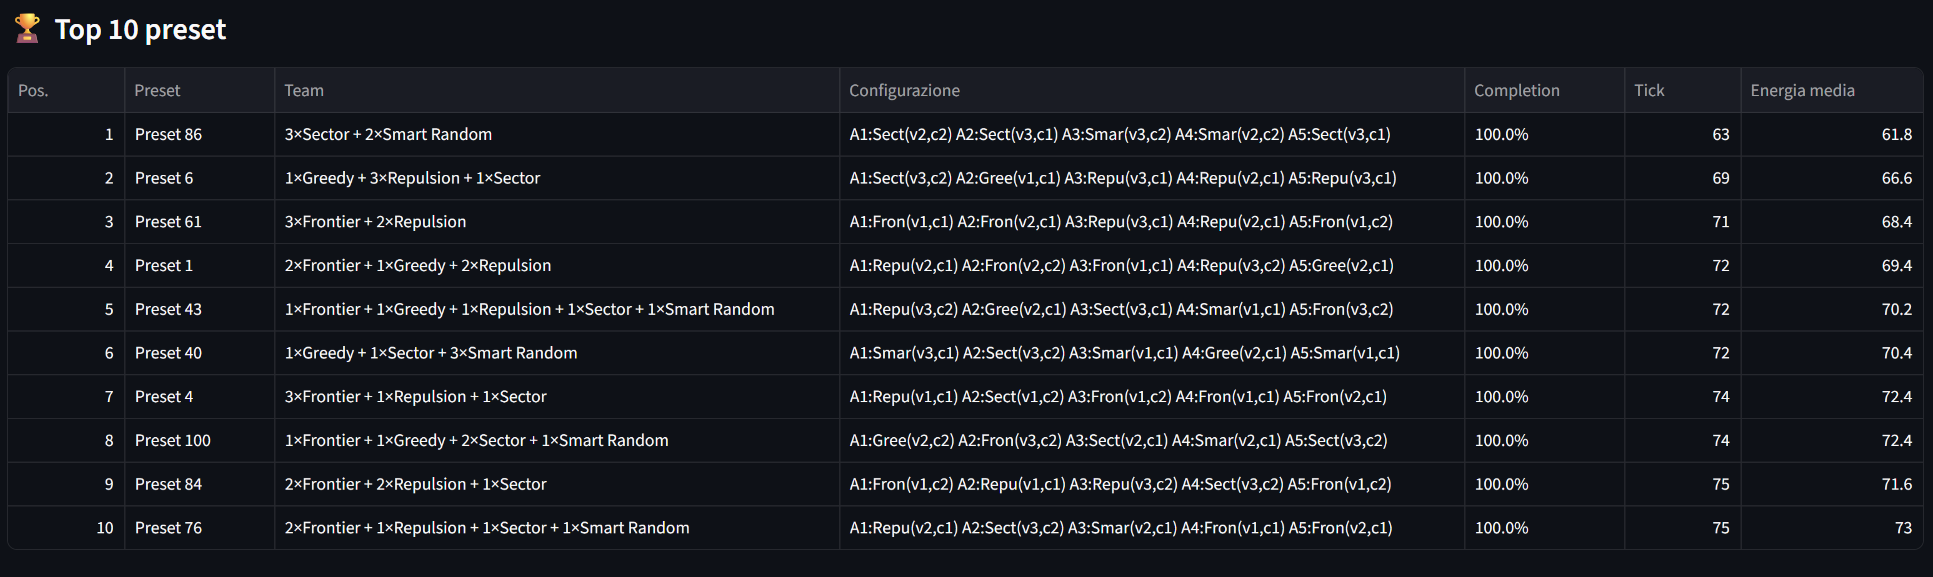
\includegraphics[width=0.92\textwidth]{../../benchmarks/B/100_sim/seed42/Images/tabelle/tabellaTop10.png}
  \caption{Mappa~B --- seed 42: classifica Top~10.}
  \label{fig:Bs42-top10}
\end{figure}

\subsubsection*{Seed 43}

\begin{figure}[H]
  \centering
  \includegraphics[width=\textwidth]{../../benchmarks/B/100_sim/seed43/Images/plot/grafico_oggetti_consegnati.png}
  \caption{Mappa~B --- seed 43: oggetti consegnati per preset.}
  \label{fig:Bs43-oggetti}
\end{figure}

\begin{figure}[H]
  \centering
  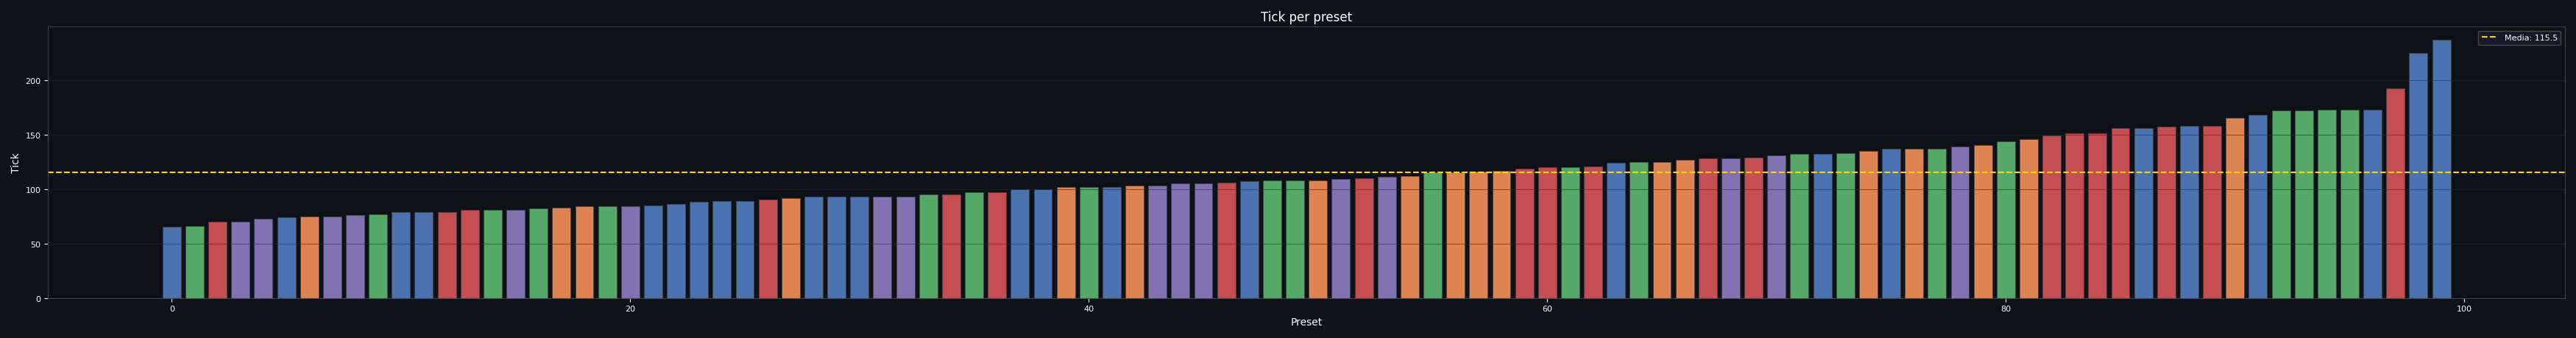
\includegraphics[width=\textwidth]{../../benchmarks/B/100_sim/seed43/Images/plot/grafico_tick_completamento.png}
  \caption{Mappa~B --- seed 43: tick di completamento per preset.}
  \label{fig:Bs43-tick}
\end{figure}

\begin{figure}[H]
  \centering
  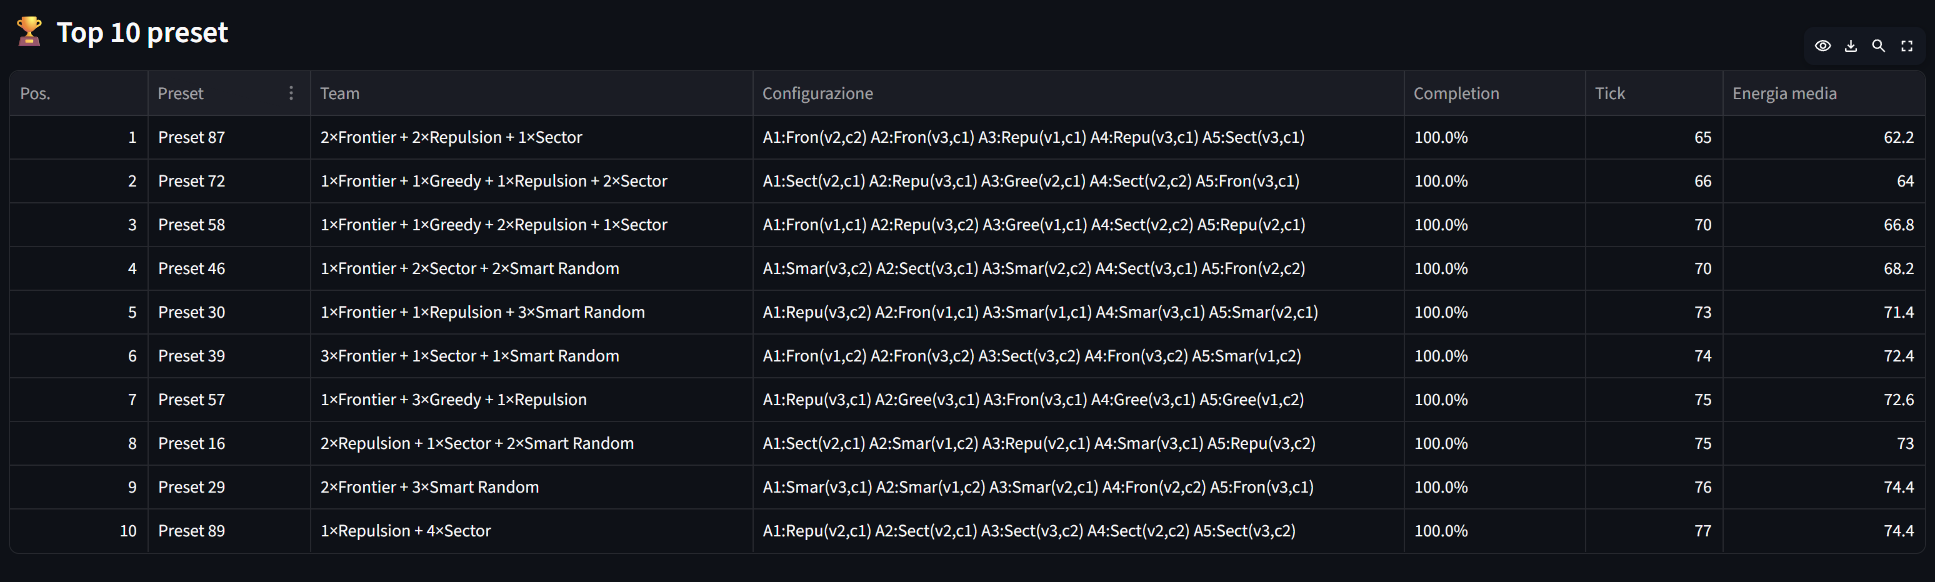
\includegraphics[width=0.92\textwidth]{../../benchmarks/B/100_sim/seed43/Images/tabelle/tabellaTop10.png}
  \caption{Mappa~B --- seed 43: classifica Top~10.}
  \label{fig:Bs43-top10}
\end{figure}

\subsubsection*{Seed 44}

\begin{figure}[H]
  \centering
  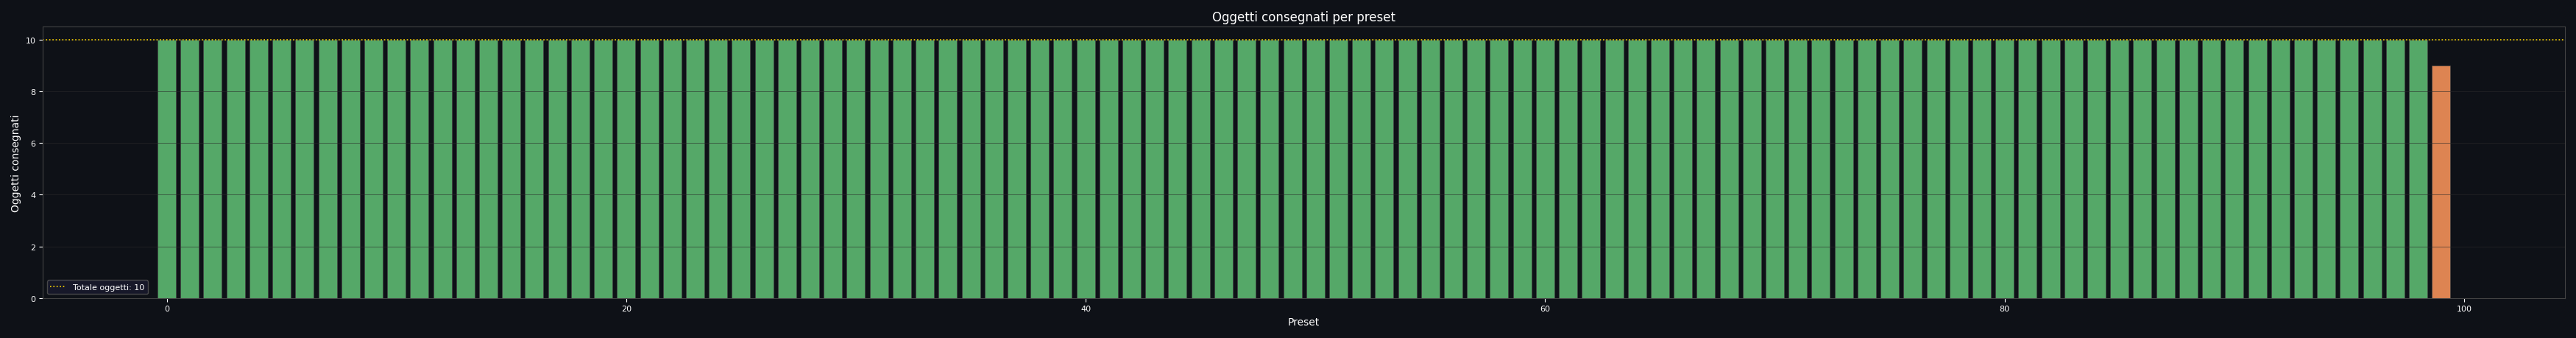
\includegraphics[width=\textwidth]{../../benchmarks/B/100_sim/seed44/Images/plot/grafico_oggetti_consegnati.png}
  \caption{Mappa~B --- seed 44: oggetti consegnati per preset.}
  \label{fig:Bs44-oggetti}
\end{figure}

\begin{figure}[H]
  \centering
  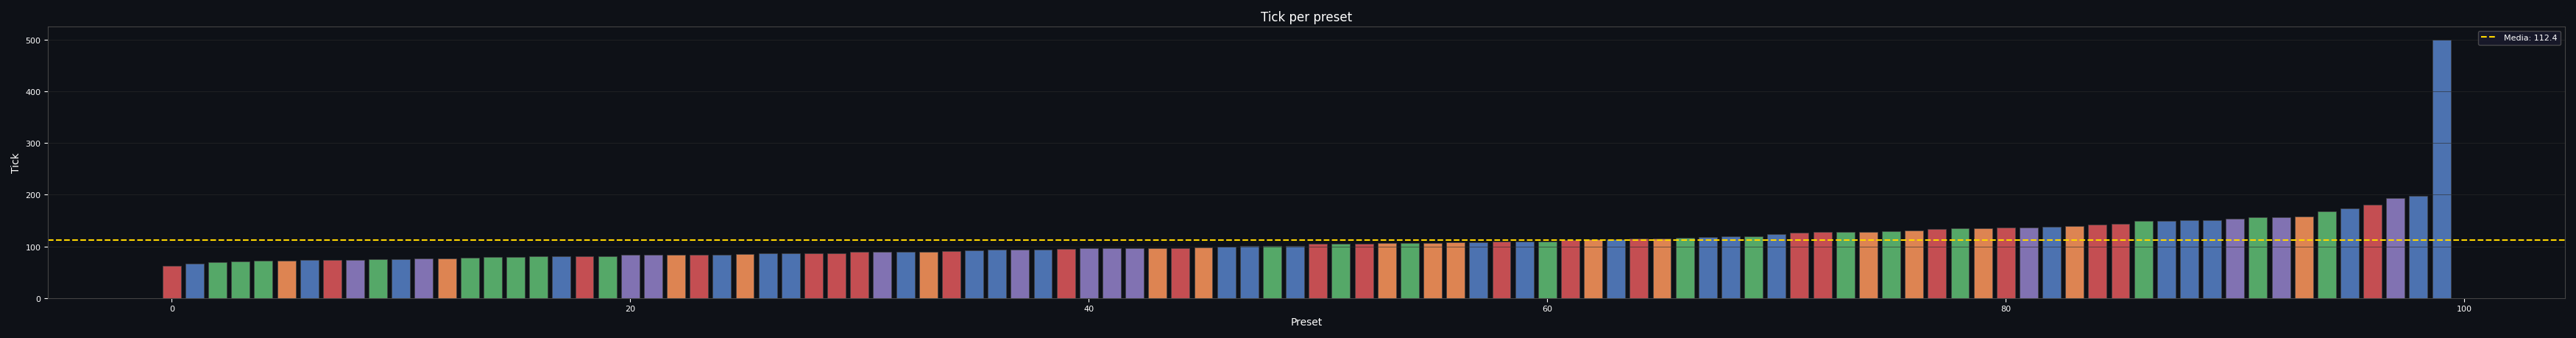
\includegraphics[width=\textwidth]{../../benchmarks/B/100_sim/seed44/Images/plot/grafico_tick_completamento.png}
  \caption{Mappa~B --- seed 44: tick di completamento per preset.}
  \label{fig:Bs44-tick}
\end{figure}

\begin{figure}[H]
  \centering
  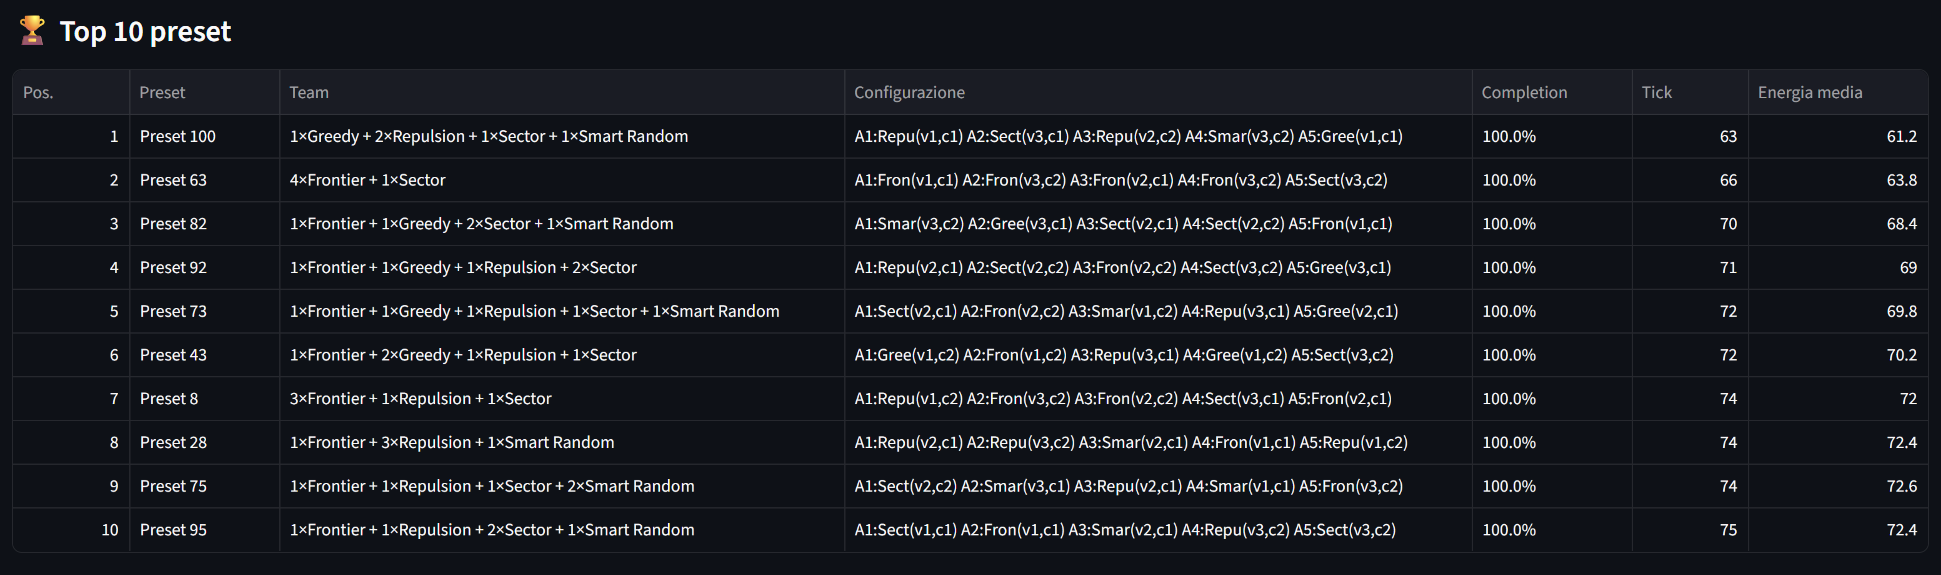
\includegraphics[width=0.92\textwidth]{../../benchmarks/B/100_sim/seed44/Images/tabelle/tabellaTop10.png}
  \caption{Mappa~B --- seed 44: classifica Top~10.}
  \label{fig:Bs44-top10}
\end{figure}

%% ═════════════════════════════════════════════════════════════════════════════
\section{Considerazioni sui risultati}
%% ═════════════════════════════════════════════════════════════════════════════

\subsection{Confronto tra le due mappe}

La Mappa~B risulta sistematicamente pi\`u semplice della Mappa~A su tutte le metriche.
Nel test esaustivo il miglior preset completa in 57~tick (contro i 77 della Mappa~A),
con un tick medio di completamento di 105{,}7 contro 162{,}9 ($-35\,\%$) e un consumo
energetico medio di 103{,}3 contro 161{,}1 ($-36\,\%$).
Il tasso di completamento sale dal 96{,}4\,\% al 99{,}6\,\%.
Questa differenza \`e attribuibile alla topologia della mappa:
una pianta pi\`u aperta riduce i cammini medi agente-oggetto e agente-magazzino,
abbassando sia i tick sia l'energia necessari.

\subsection{Impatto della strategia dominante}

Analizzando i 32.768 preset completati per strategia dominante
(la strategia che compare pi\`u volte nel team di 5 agenti), emerge una chiara
differenza tra le due mappe:

\begin{itemize}
  \item \textbf{Mappa~A}: le quattro strategie ottengono tick medi molto simili
        (Repulsion 158{,}7, Greedy 161{,}5, Sector 163{,}0, Frontier 168{,}5),
        con Repulsion leggermente avvantaggiata.
        Nella Top~10, Sector domina con 17 assegnazioni su 50, seguito da
        Greedy~(12) e Repulsion~(11).
    \item \textbf{Mappa~B}: Repulsion emerge nettamente come strategia migliore
      (101{,}5 tick medi, $-9\,\%$ rispetto a Frontier).
        Nella Top~10 compare 23 volte su 50, contro 13 di Sector e 10 di Frontier.
\end{itemize}

\textit{Nota sulla posizione sistemática di Sector nei team Top~10:}
Sector appare sistematicamente inserito in 4\textsuperscript{a} posizione
(indice agente 3) nei team Top~10 di entrambe le mappe. Questo fenomeno non \`e casuale:
la strategia Sector divide la griglia in bande orizzontali assegnate agli agenti in base a
$\texttt{agent\_id} \bmod N$. Agenti con ID inferiore occupano bande pi\`u alte e procedono
verso il basso in modo sistematico. Posizionare Sector in 4\textsuperscript{a} posizione
minimizza la sovrapposizione con gli altri agenti: se Sector avesse ID inferiore,
la sua banda occuperrebbe spazio sin dall'inizio della mappa, potenzialmente entrando
in conflitto con le traiettorie delle altre strategie. Questa configurazione emerge
naturalmente dall'ottimizzazione, riflettendo il trade-off tra copertura sistematica
di Sector e flessibilità delle altre strategie nei team misti.

\subsection{Team eterogenei vs omogenei}

I team omogenei (tutti e 5 gli agenti con la stessa strategia) rappresentano
solo 128 dei 32.768 preset per ciascuna mappa. I risultati sono eloquenti:

\begin{itemize}
  \item \textbf{Mappa~A}: team omogenei completano nel 96{,}9\,\% dei casi con una media
        di 172{,}5~tick; team eterogenei completano nel 96{,}4\,\% con 162{,}9~tick
        e ottengono il record assoluto di 77~tick. Nessun team omogeneo scende sotto i 99~tick.
  \item \textbf{Mappa~B}: team omogenei completano nel 100\,\% dei casi con 102{,}3~tick
        medi, ma il miglior risultato \`e 64~tick; i team eterogenei raggiungono 57~tick.
\end{itemize}

In entrambe le mappe il \textbf{miglior preset assoluto \`e sempre eterogeneo}. Un team
misto beneficia della complementarit\`a tra le strategie: Sector fornisce copertura
sistematica, Repulsion garantisce dispersione, Greedy ottimizza i percorsi verso i
magazzini e Frontier esplora le zone residue.

\subsection{Impatto del raggio di visibilit\`a}

Raggruppando i preset completati per raggio di visibilit\`a medio del team ($\bar{v}_r$), si
osserva un trend diverso nelle due mappe:

\begin{itemize}
  \item \textbf{Mappa~A}: i tick medi calano da 175{,}1 ($\bar{v}_r=2{,}0$) a 152{,}6
        ($\bar{v}_r=2{,}8$), ma risalgono a 162{,}9 per $\bar{v}_r=3{,}0$.
        Il raggio ottimale si colloca intorno a $\bar{v}_r \approx 2{,}6$--$2{,}8$:
        un campo visivo troppo ampio aumenta il costo computazionale del ray casting
        senza aggiungere informazione utile in corridoi stretti.
  \item \textbf{Mappa~B}: i tick calano monotonicamente da 116{,}1 ($\bar{v}_r=2{,}0$)
        a 96{,}7 ($\bar{v}_r=3{,}0$).
        Su una mappa aperta un raggio maggiore \`e sempre vantaggioso perch\'e
        incrementa direttamente l'area scansionata ad ogni tick.
\end{itemize}

Nonostante queste differenze, i Top~10 di entrambe le mappe mantengono un mix di raggi~2 e~3,
suggerendo che la diversit\`a percettiva nel team contribuisce alla robustezza.

\subsection{Robustezza ai seed casuali}

Il test randomizzato con 3~seed indipendenti consente di stimare la sensibilit\`a al rumore
stocastico. I risultati sono stabili:

\begin{itemize}
  \item \textbf{Mappa~A}: i tick medi oscillano tra 155{,}5 e 163{,}1 nei tre seed,
        con una variazione massima del $\pm 2{,}4\,\%$ rispetto alla media.
        Il tasso di completamento \`e costante ($96$--$97\,\%$).
  \item \textbf{Mappa~B}: i tick oscillano tra 108{,}5 e 115{,}5 ($\pm 3{,}1\,\%$).
        Il completamento \`e quasi perfetto ($99$--$100\,\%$) su tutti e tre i seed.
\end{itemize}

La bassa varianza inter-seed conferma che le prestazioni osservate dipendono prevalentemente
dalla configurazione del team e dalla topologia della mappa, non dalla specifica
distribuzione casuale degli oggetti.

\subsection{Riepilogo}

\begin{enumerate}
  \item La topologia della mappa \`e il fattore pi\`u influente: mappe aperte (B) sono
        risolvibili il 35\,\% pi\`u velocemente di mappe strutturate (A).
  \item I team eterogenei battono sistematicamente quelli omogenei nei tempi migliori,
        sfruttando la complementarit\`a tra strategie diverse.
  \item Repulsion \`e la strategia pi\`u performante su mappe aperte;
        Sector e Greedy risultano competitivi su mappe con corridoi.
  \item Un raggio di visibilit\`a elevato \`e sempre vantaggioso su mappe aperte,
        mentre su mappe strutturate esiste un punto di rendimento decrescente
        intorno a $\bar{v}_r \approx 2{,}6$--$2{,}8$.
  \item Il sistema mostra buona robustezza statistica, con variazioni contenute
        al variare del seed casuale.
\end{enumerate}

\newpage
% ═════════════════════════════════════════════════════════════════════════════
\subsection{Riepilogo delle euristiche utilizzate}
% ═════════════════════════════════════════════════════════════════════════════

Il sistema impiega un insieme composito di euristiche, ciascuna con un ruolo specifico
nel coordinamento e nella decisione dei team multi-agente:

\begin{description}
  \item[\textbf{Ray-casting (Bresenham)}]
        Calcola la visione dell'agente entro raggio $v_r$ considerando l'occlusione
        da muri. Base della percezione distribuita.
  
  \item[\textbf{Coverage targets}]
        Fornisce tre livelli di priorit\`a per l'esplorazione: celle inesplorate,
        celle stale (non visitate di recente), pattugliamento. Guida tutte le strategie
        verso aree di maggior interesse.
  
  \item[\textbf{Guadagno informativo (\textit{info\_gain})}]
        Per una cella candidata~$t$, conta le celle non ancora viste che l'agente
        osserverebbe da quella posizione:
        $$\text{info\_gain}(t) = \bigl|\,\{(r,c) : |r - t_r| + |c - t_c| \le v_r
        \;\wedge\; (r,c) \notin \text{seen\_cells}\}\,\bigr|$$
        Usato da Smart Random Walk e Greedy per favorire mosse verso aree dense
        di celle inesplorate.
  
  \item[\textbf{Scelta dell'ingresso di consegna (Costo dinamico)}]
        Per un ingresso~$e$ combina distanza, congestione e prenotazioni:
        $$C(e) \;=\; d(\text{agent},\,e) \;+\; 4{,}5\cdot Q_{\text{local}}
        \;+\; 1{,}5\cdot R_{\text{reserved}} \;+\; \varepsilon_{\text{tie}}$$
        dove $Q_{\text{local}}$ sono gli agenti noti entro raggio~2 e $R_{\text{reserved}}$
        \`e il numero di prenotazioni attive. Scelta rideterminata a ogni tick, con hysteresis
        del 20\% per evitare oscillazioni.
  
  \item[\textbf{Separazione (Repulsion)}]
        Massimizza la distanza media dagli agenti noti:
        $$\text{score}(t) = \frac{1}{|\mathcal{A}|}\sum_{a \in \mathcal{A}} d(t, a) - d(\text{agent}, t)$$
        Induce dispersione naturale senza comunicazione esplicita; efficace su mappe aperte.
  
  \item[\textbf{Frontiere (\textit{frontier-based})}]
        Identifica celle visitate che confinano con celle non visitate. Classico
        approccio all'esplorazione sistematica con A* per il raggiungimento.
  
  \item[\textbf{Costo composito (Greedy)}]
        Minimizza il costo composito di esplorazione:
        $$\text{cost}(t) = d(\text{agent}, t) + d(t, \text{wh}_{\text{nearest}}) - \text{info\_gain}(t)$$
        Bilancia distanza, prossimit\`a al magazzino pi\`u vicino, e guadagno informativo.
        Produce bias verso zone inesplorate ma raggiungibili efficientemente.
  
  \item[\textbf{Pattern a banda (Sector)}]
        Divide la griglia in bande orizzontali assegnate per $\texttt{agent\_id} \bmod N$.
        Garantisce copertura sistematica e uniforme senza comunicazione di coordinamento.
  
  \item[\textbf{Punteggio multi-criterio (Smart Random Walk)}]
        Calcola il punteggio come somma pesata di cinque criteri:
        $$\text{score}(n) = w_{\text{info}} \cdot \text{info\_gain}(n) + w_{\text{stale}} \cdot \text{age}(n)
        - w_{\text{revisit}} \cdot \text{penalty}(n) + w_{\text{sep}} \cdot \text{separation}(n) + \mathcal{U}(0,\,0{,}3)$$
        con pesi: $w_{\text{info}}=1{,}2$, $w_{\text{stale}}=0{,}8$, $w_{\text{sep}}=0{,}5$, $w_{\text{revisit}}=1{,}0$.
        Softmax per selezione probabilistica.
  
  \item[\textbf{Costo-beneficio con hysteresis}]
        Applica un 20\% di soglia di miglioramento prima di cambiare destinazione di consegna
        (lock di 8~tick). Riduce oscillazioni e overhead comunicativo.
  
  \item[\textbf{Pathfinding A*}]
        Ricerca del percorso pi\`u breve verso target con euristica Manhattan. Le celle occupate
        da altri agenti vengono passate come set di celle bloccate per evitare collisioni.
        Supporta modalit\`a specifica per transito attraverso il magazzino durante consegna.
  
  \item[\textbf{Finestra di validit\`a temporale}]
        Le posizioni degli agenti noti sono valide per 5~tick. Informazioni pi\`u vecchie
        vengono scartate durante la pianificazione locale per evitare collisioni con
        agenti spostati nel frattempo. Permette agli agenti di gestire un modello parziale
        del sistema pur mantenendo sicurezza.
  
  \item[\textbf{Stale detection e pulizia}]
        Celle non visitate entro $\max(8,\,N/2)$ tick vengono riclassificate come \textit{stale}
        nei coverage targets. Gli oggetti rimossi dalla visibilità diretta vengono eliminati da
        \texttt{known\_objects} per evitare ricerche fantasma. Mantiene coerenza tra percezione
        e memoria locale.
  
  \item[\textbf{Gossip protocol distribuito}]
        Ad ogni comunicazione, gli agenti scambiano bidirezionalmente: mappa locale, oggetti noti,
        posizioni di agenti conosciuti (merge con timestamp), prenotazioni di consegna.
        Non esiste canale broadcast globale; la conoscenza si propaga per contatto diretto,
        creando un effetto di diffusione graduale che favorisce robustezza e decentralizzazione.
  
  \item[\textbf{Priorit\`a deterministiche nelle collisioni}]
        In caso di conflitto per la stessa cella: priorità a chi trasporta un oggetto;
        a parità di stato, vince l'agente con ID inferiore. Garantisce risoluzione senza
        deadlock e comportamento prevedibile nel debugging. Gli agenti bloccati restano
        fermi e riprovano al prossimo tick.
  
  \item[\textbf{Protezione delle porte magazzino}]
        Celle \texttt{ENTRANCE} e \texttt{EXIT} sono automaticamente protette come celle bloccate
        durante la pianificazione A*. Impedisce che vengano usate come scorciatoie o transiti
        intermedi, riducendo congestione e garantendo che siano raggiunte solo come destinazione
        finale di un percorso.
\end{description}

